\documentclass[10pt,a4paper]{article}

\usepackage[utf8]{inputenc}
\usepackage[T1]{fontenc}
\usepackage{amsmath,amssymb,amsfonts}
\usepackage{graphicx}
\usepackage{hyperref}
\usepackage{algorithm}
\usepackage{algpseudocode}
\usepackage{multicol}
\usepackage{geometry}
\usepackage{cite}
\usepackage{authblk}
\usepackage{amsmath, mathtools, empheq}

% Page layout
\geometry{margin=2cm}

% Title page
\title{\Large\textbf{TPTT: Transforming Pretrained Transformers into Titans}}
\author{\large Fabien Furfaro\thanks{\texttt{fabien.furfaro@gmail.com}}}
\date{\large 2025}

\begin{document}

\maketitle

\begin{abstract}
Recent advances in large language models (LLMs) have led to remarkable progress in natural language processing, but their computational and memory demands remain a significant challenge, particularly for long-context inference. We introduce TPTT (Transforming Pretrained Transformers into Titans), a novel framework for enhancing pretrained Transformers models with efficient linearized attention mechanisms and advanced memory management. TPTT employs techniques such as Memory as Gate (MaG) and mixed linearized attention (LiZA). It is fully compatible with the Hugging Face Transformers library, enabling seamless adaptation of any causal LLM through parameter-efficient fine-tuning (LoRA) without full retraining. We show the effectiveness of TPTT on the MMLU benchmark with models of approximately 1 billion parameters, observing substantial improvements in both efficiency and accuracy. For instance, Titans-Llama-3.2-1B achieves a 20\% increase in Exact Match (EM) over its baseline. Statistical analyses and comparisons with recent state-of-the-art methods confirm the practical scalability and robustness of TPTT. The source code is available at \url{https://github.com/fabienfrfr/tptt} and the Python package at \url{https://pypi.org/project/tptt/}.
\end{abstract}


\begin{figure}[ht]
    \centering
    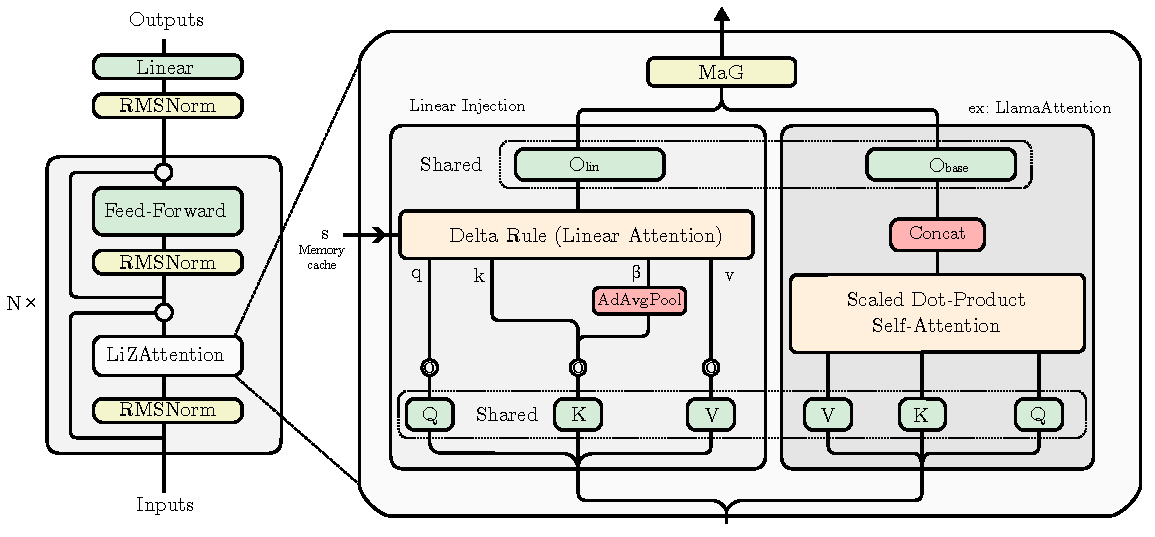
\includegraphics[width=0.8\linewidth]{fig.pdf}
    \caption{Overview of the TPTT architecture. On the left, the diagram illustrates a decoder-only architecture where linear attention is injected in parallel of vanilla attention (LiZAttention). On the right, the detailed architecture of the linearized attention mechanism is depicted, highlighting the shared weights for query (Q), key (K), value (V), and output (O) projections. It also shows the management of the state memory (S) and the combination of outputs through the Memory as Gate (MaG) weighting mechanism. The state can be unlinear between chunk. The diagram emphasizes the integration of linearized attention mechanisms and advanced memory management techniques, such as DeltaProduct and AdaptativeAvgPool1D, contributing to processing and output generation.}
    \label{fig:approach_overview}
\end{figure}


\section{Introduction}

The success of transformer-based large language models (LLMs)~\cite{vaswani2017attention, mann2020language} has revolutionized natural language processing (NLP), enabling unprecedented progress across a wide range of tasks. However, the quadratic computational complexity and substantial memory requirements of the standard self-attention mechanism remain a significant bottleneck, particularly for long-context inference. 

To address these challenges, recent research has explored several directions. Efficient attention mechanisms~\cite{katharopoulos2020transformers, yang2024parallelizing} have been proposed to reduce the complexity of self-attention from quadratic to linear or near-linear, making it more tractable for long sequences. Recurrent architectures and internal memory mechanisms~\cite{mercat2024linearizing, behrouz2024titans} have also been developed to enhance the model's ability to capture long-range dependencies, drawing inspiration from cognitive memory in biological systems rather than hardware memory. Additionally, parameter-efficient fine-tuning approaches such as LoRA~\cite{hu2022lora} allow for the adaptation of large pretrained models to new tasks without the need for full retraining.

\section{Related Work}

Despite these advances, most existing methods require significant architectural modifications or training from scratch, which limits their applicability to already pretrained models. For example, solutions like FlashAttention~\cite{dao2023flashattention} and Mamba~\cite{gu2023mamba} focus on efficient architectures, while others such as LoLCat~\cite{zhang2024lolcats} and Liger~\cite{lan2025liger} convert standard attention to linearized forms; notably, Liger exploits similar properties to those leveraged in this work, but does not rely on explicit linearization injection.

In this work, we introduce TPTT (Transforming Pretrained Transformers into Titans), a framework that transforms pretrained Transformers models into efficient and scalable architectures by incorporating linearized attention mechanisms and advanced internal memory augmentation. TPTT leverages techniques such as Memory as Gate (MaG) and mixed linearized attention (LiZA), drawing inspiration from the Titans architecture~\cite{behrouz2024titans}. Our approach is fully compatible with existing frameworks and enables rapid adaptation of any causal LLM to long-context tasks via parameter-efficient fine-tuning with LoRA~\cite{hu2022lora}, without requiring full retraining. The goal is to unlock the potential of already trained models by equipping them with memory-augmented capabilities through lightweight adaptation.

\section{Methodology}

\subsection{Linearized Attention Mechanisms}

Standard self-attention in transformers computes pairwise interactions between all tokens, resulting in quadratic complexity with respect to sequence length~\cite{vaswani2017attention}. To address this, linearized attention mechanisms approximate the softmax attention using linear operations, typically by projecting queries and keys through a feature map $\phi$~\cite{katharopoulos2020transformers, wang2020linformer, mercat2024linearizing, yang2024parallelizing}. This reduces computational and memory costs, enabling efficient processing of long sequences while maintaining modeling power~\cite{gu2023mamba, dao2023flashattention, zhang2024lolcats, lan2025liger}. The output of softmax attention for an input sequence $\mathbf{X} = \{\mathbf{x}_1, \dots, \mathbf{x}_T\} \in \mathbb{R}^{T \times D}$ is:
\begin{equation}
\mathbf{Q}, \mathbf{K}, \mathbf{V} = \mathbf{X}\mathbf{W}_Q, \mathbf{X}\mathbf{W}_K, \mathbf{X}\mathbf{W}_V
\end{equation}
\begin{equation}
\mathbf{O}_{\text{base}} = \text{Softmax}\left(\frac{\mathbf{Q}\mathbf{K}^\top}{\sqrt{D}}\right)\mathbf{V}
\end{equation}
In linear attention, this is approximated as:
\begin{equation}
\mathbf{O}_{\text{lin}, (t)} = 
\frac{
\phi(\mathbf{q}_t)^\top \left( \sum_{i=1}^t \phi(\mathbf{k}_i, \beta_i)\, \mathbf{v}_i^\top \right)}{
\phi(\mathbf{q}_t)^\top \left( \sum_{i=1}^t \phi(\mathbf{k}_i, \beta_i) \right)} 
= \frac{\phi(\mathbf{q}_t)^\top S_t}{\phi(\mathbf{q}_t)^\top z_t}
\end{equation}

where $\mathbf{q}_t$, $\mathbf{k}_i$, and $\mathbf{v}_i$ are the query, key, and value vectors at positions $t$ and $i$, respectively, and $\beta_i$ is a gating vector (or scalar) modulating the keys and values. The function $\phi$ denotes a feature mapping, such as ELU or kernel approximations~\cite{wang2020linformer}. In this work, $\beta_i$ is constructed from average pooling of the keys and values.

\subsection{Memory as Gate (MaG)}

To further enhance long-range dependency modeling, we introduce an internal memory augmentation mechanism, Memory as Gate (MaG), inspired by the Titans architecture~\cite{behrouz2024titans}. This mechanism enables the model to store and recall contextual information over extended sequences, analogous to cognitive memory (persistence, surprise, etc.). MaG combines the outputs of standard and linearized attention using a weighting parameter:
\begin{equation}
\mathbf{O} = \alpha \cdot \mathbf{O}_{\text{lin}} + (1-\alpha) \cdot \mathbf{O}_{\text{base}}
\end{equation}
where $\alpha \in [0,1]$ is adapted during training. This allows the model to leverage both the efficiency of linear attention and the expressivity of softmax attention, and can be seen as a form of memory-augmented gating~\cite{behrouz2024titans, mercat2024linearizing, munkhdalai2024leave}.

\subsection{Parallel Delta Product Modeling}

In this work, the feature mapping function of linear attention is based on the DeltaProduct operator, which generalizes the Delta rule to achieve higher expressivity while maintaining efficient parallelization. This approach addresses the limitations of linear recurrent architectures, which struggled to balance state-tracking power and hardware efficiency~\cite{siems2025deltaproduct, yang2024parallelizing}.

The Delta rule~\cite{rumelhart1986learning}, as used in associative memory models, updates the memory state sequentially as:
\begin{equation}
    \mathbf{S}_t = \mathbf{S}_{t-1} + \beta_t \left( \mathbf{v}_t - \mathbf{S}_{t-1} \mathbf{k}_t \right) \mathbf{k}_t^\top
    \qquad \text{(sequential, delta rule)}
\end{equation}
where $\mathbf{S}_t$ is the memory state at time $t$, $\mathbf{k}_t$ and $\mathbf{v}_t$ are the key and value, and $\beta_t$ is a gating parameter. This update is inherently sequential and thus not directly parallelizable.

\paragraph{DeltaNet: Parallelization via Householder Product}

DeltaNet~\cite{yang2024parallelizing} enables efficient parallelization by chunking the sequence and vectorizing the update within each chunk using a compact product of Householder matrices. For a chunk of size $C$, the intra-chunk parallel update (order $n=1$) is:
\begin{equation}
    \mathbf{S}_{[t,\,t+C-1]} = \mathbf{S}_{t-1} + \mathbf{K}^\top
    \left[ \mathbf{T}^{-1}
    \left( \mathbf{V} \odot \boldsymbol{\beta} - (\mathbf{K} \odot \boldsymbol{\beta}) \mathbf{S}_{t-1} \right) \right]
    \qquad \text{(parallel, intra-chunk, order 1)}
\end{equation}
where $\mathbf{K} \in \mathbb{R}^{C \times d}$ and $\mathbf{V} \in \mathbb{R}^{C \times d}$ are the stacked keys and values in the chunk, $\boldsymbol{\beta} \in \mathbb{R}^{C \times 1}$ is the gating vector, $\odot$ denotes element-wise multiplication, and
\begin{equation}
    \mathbf{T} = \mathbf{I} - \mathrm{tril}\left((\mathbf{K} \odot \boldsymbol{\beta}) \mathbf{K}^\top, -1\right)
\end{equation}
with $\mathrm{tril}(\cdot, -1)$ extracting the strictly lower triangular part. This chunkwise formulation enables efficient batched computation on modern hardware by removing sequential dependencies within each chunk~\cite{yang2024parallelizing, siems2025deltaproduct}. To further increase expressivity, a non-linearity $\phi$ (e.g., GELU or tanh) can be applied to the state update:
\begin{equation}
    \mathbf{S}_t = \phi(\mathbf{S}_{t-1} + \beta_t \left( \mathbf{v}_t - \mathbf{S}_{t-1} \mathbf{k}_t \right) \mathbf{k}_t^\top)
\end{equation}

\paragraph{DeltaProduct: Generalization to Higher Order}

DeltaProduct~\cite{siems2025deltaproduct} extends this approach by applying $n$ rank-1 corrections per token, corresponding to a product of $n$ Householder-like transformations. For each position $i$, the state update is defined recursively as:
\begin{equation}
    H_{i,j} = H_{i,j-1} - \beta_{i,j} (H_{i,j-1} \mathbf{k}_{i,j} - \mathbf{v}_{i,j}) \mathbf{k}_{i,j}^\top
    \qquad \text{for } j=1,\ldots,n
\end{equation}
where $H_{i,0} = H_{i-1}$ and $H_{i,n} = H_i$. This can be unrolled as:
\begin{align}
    H_i &= A(\mathbf{x}_i) H_{i-1} + B(\mathbf{x}_i) \\
    A(\mathbf{x}_i) &= \prod_{j=1}^n \left( \mathbf{I} - \beta_{i,j} \mathbf{k}_{i,j} \mathbf{k}_{i,j}^\top \right) \\
    B(\mathbf{x}_i) &= \sum_{j=1}^n \left( \prod_{k=j+1}^n \left( \mathbf{I} - \beta_{i,k} \mathbf{k}_{i,k} \mathbf{k}_{i,k}^\top \right) \right) \beta_{i,j} \mathbf{k}_{i,j} \mathbf{v}_{i,j}^\top
\end{align}
where $\mathbf{k}_{i,j}$, $\mathbf{v}_{i,j}$, and $\beta_{i,j}$ are the key, value, and gate for the $j$-th virtual token at position $i$. 

To construct the $n$ virtual tokens per real token, we use a binomial finite difference expansion (derivative trick), as follows:
\begin{equation}
    \mathbf{x}^{(m)}_t = \sum_{k=0}^m (-1)^k \binom{m}{k} \mathbf{x}_{t-k}
    \qquad \text{for } m=0,\ldots,n-1
\end{equation}
where $\mathbf{x}^{(m)}_t$ is the $m$-th discrete derivative (virtual token) at position $t$~\cite{behrouz2025s}.

The corresponding chunkwise parallel update is:
\begin{align}
    \mathbf{S}_{[t,\,t+C-1]} = \mathbf{S}_{t-1} + \mathbf{K}_h^\top
    \left[ \mathbf{T}_h^{-1}
    \left( \mathbf{V}_h \odot \boldsymbol{\beta}_h - (\mathbf{K}_h \odot \boldsymbol{\beta}_h) \mathbf{S}_{t-1} \right) \right]
    \qquad \text{(parallel, intra-chunk, order $n$)}
\end{align}
where, for each Householder step $h$, $\mathbf{K}_h, \mathbf{V}_h \in \mathbb{R}^{(nC) \times d}$ and $\boldsymbol{\beta}_h \in \mathbb{R}^{(nC) \times 1}$ are the keys, values, and gates for the $h$-th virtual token within the chunk, and
\begin{equation}
    \mathbf{T}_h = \mathbf{I} - \mathrm{tril}\left((\mathbf{K}_h \odot \boldsymbol{\beta}_h) \mathbf{K}_h^\top, -1\right).
\end{equation}

This matches our implementation: the input is expanded into $n$ virtual tokens per real token using the derivative trick, and all $\mathbf{T}_h$ are inverted in parallel for efficient batched computation on GPU. The final state $\mathbf{S}_{t+C-1}$ initializes the next chunk.

\paragraph{Expressivity and Theoretical Properties.}
By increasing the order $n$, DeltaProduct interpolates between the original DeltaNet ($n=1$) and a dense state transition. Notably, DeltaProduct of order $n=2$ achieves a level of expressivity comparable to the Titans model and can solve algorithmic problems beyond the class $\mathrm{TC}^0$ (such as parity)~\cite{siems2025deltaproduct, merrill2024illusion}. This is in contrast to diagonal or single-rank updates, which are fundamentally limited in this regard. DeltaProduct thus provides a tunable trade-off between efficiency and expressivity, while retaining the hardware efficiency of the chunkwise parallel algorithm.



\subsection{Integration with Pretrained Models}

Our approach injects linearized attention and memory augmentation modules into pretrained Transformers models. The process involves:
\begin{enumerate}
    \item \textbf{Identification of Target Modules:} Key attention layers to be modified are identified using tools such as \textit{get\_tptt\_model}.
    \item \textbf{Modification of Attention Layers:} These layers are replaced or extended with the proposed \textit{LiZAttention} module, which implements both linear and softmax attention with linear projection weigth sharing and MaG.
    \item \textbf{Training and Fine-Tuning:} The modified model is fine-tuned using parameter-efficient methods such as LoRA~\cite{hu2022lora}, ensuring optimal adaptation to the new mechanisms without full retraining.
\end{enumerate}
This procedure enables the transformation of any causal pretrained LLM into a memory-augmented, efficient architecture with minimal overhead, that without any new layers.


\subsection{LiZAttention Module}

The \texttt{LiZAttention} module is a core component of the TPTT architecture, designed to synergistically combine linearized attention and standard (softmax) attention mechanisms. This hybrid approach leverages the computational efficiency of linear attention while retaining the expressivity of vanilla attention. To support long-context inference, \texttt{LiZAttention} maintains a cache of intermediate states and implements a recurrent information mechanism for efficient internal memory management~\cite{katharopoulos2020transformers}.

\begin{algorithm}[H]
\caption{LiZAttention Forward Pass}
\label{alg:lizattention}
\begin{algorithmic}[1]
\Require $\text{hidden\_states} \in \mathbb{R}^{B \times L \times D}$ \Comment{Batch size $B$, sequence length $L$, embedding dim $D$}
\Require $\text{mask}$ \Comment{Attention mask for padding/causality}
\State \textbf{Projection:}
    \Statex \hspace{1em} Compute queries $q$, keys $k$, values $v$ via learned projections:
    \Statex \hspace{1em} $q \in \mathbb{R}^{B \times H \times L \times d_h}$, $k, v \in \mathbb{R}^{B \times H_k \times L \times d_h}$
\State \textbf{Apply Attention Mask:}
    \Statex \hspace{1em} Apply $\text{mask}$ to $k$ and $v$ to handle padding and restrict attention.
\State \textbf{Linear Attention:}
    \Statex \hspace{1em} Compute linear attention output $o_{\mathrm{lin}}$ using a feature map $\phi$:
    \Statex \hspace{1em} $o_{\mathrm{lin}}[t] = \frac{\sum_{i=1}^{t} \phi(q_t)^\top \phi(k_i) v_i}{\sum_{i=1}^{t} \phi(q_t)^\top \phi(k_i)}$
    \Statex \hspace{1em} Store intermediate states in a memory cache for recurrent information.
\State \textbf{Vanilla (Softmax) Attention:}
    \Statex \hspace{1em} Compute standard self-attention output $o_{\mathrm{base}}$ (optionally truncated for long sequences):
    \Statex \hspace{1em} $o_{\mathrm{base}} = \text{Softmax}\left(\frac{q k^\top}{\sqrt{d_h}}\right) v$
\State \textbf{Combine Outputs (Memory as Gate):}
    \Statex \hspace{1em} Compute final output using a learnable gating parameter $\alpha$:
    \Statex \hspace{1em} $o = \alpha \cdot o_{\mathrm{lin}} + (1-\alpha) \cdot o_{\mathrm{base}}$
\State \Return $o \in \mathbb{R}^{B \times L \times D}$
\end{algorithmic}
\end{algorithm}

\subsubsection{Efficient Internal Memory Management}

The cache of intermediate states maintained by \texttt{LiZAttention} enables a recurrent information, efficiently supporting long-context inference without excessive computational overhead~\cite{katharopoulos2020transformers}. This approach allows the model to scale to longer sequences, leveraging both local and global context.

\section{Training Procedure}

\subsection{Parameter-Efficient Fine-Tuning with LoRA}

To adapt the TPTT architecture to downstream tasks, we employ Low-Rank Adaptation (LoRA)~\cite{hu2022lora, lora_hf}, a parameter-efficient fine-tuning technique that injects trainable low-rank matrices into selected projection layers while freezing the original model weights. This approach reduces the number of trainable parameters and memory requirements, while maintaining performance comparable to full fine-tuning~\cite{hu2022lora, lora_hf}. LoRA is configured with a rank of 8, $\alpha=16$, and a dropout rate of 0.05. Fine-tuning targets the main projection modules, specifically \texttt{[q\_proj, k\_proj, v\_proj, o\_proj]} for Llama/Mistral and \texttt{[qkv\_proj, out\_proj]} for OpenELM~\cite{lora_hf}.

\subsection{Dynamic Memory as Gate Scheduling (LiZA MaG Callback)}

A important component of the training process is the LiZA MaG callback, which dynamically adjusts the Memory as Gate (MaG) weighting parameter during training. The MaG weight is initialized at 0.01 and linearly increased to 0.5 over the first 100 steps, facilitating a smooth transition from reliance on vanilla (softmax) attention to linearized attention. This schedule allows the model to effectively balance the two attention mechanisms, optimizing performance throughout training. The callback is integrated directly into the training loop, ensuring adaptive control of the MaG parameter and enhancing the model's adaptability and efficiency.


\section{Experiments and Results}

\subsection{Experimental Setup}

We evaluated the TPTT library on several pretrained language models with approximately 1 billion parameters, using the MMLU benchmark~\cite{hendrycks2020measuring} as the primary evaluation suite. Training was conducted on 500 samples from the \texttt{yahma/alpaca-cleaned} dataset~\cite{taori2023alpaca} for 5 epochs, with a maximum sequence length of 384 tokens, a batch size of 3, and a learning rate of $5 \times 10^{-4}$. Mixed precision training and gradient clipping at 1.0 were employed to optimize computational efficiency and stability. All experiments were performed on NVIDIA Tesla T4 GPUs (Kaggle platform). The trained models and detailed metrics are publicly available on the Hugging Face Model Hub\footnote{\url{https://huggingface.co/ffurfaro/}}, with full training logs accessible via Hugging Face TensorBoard.

\subsection{Training Results}

Table~\ref{tab:training-metrics} summarizes the training performance metrics for various TPTT models. The results indicate consistent and efficient learning across architectures, by low final loss values and stable gradient norms. The use of Low-Rank Adaptation (LoRA) and the Memory as Gate (MaG) mechanism shows effective in optimizing training dynamics and convergence.

\begin{table}[h!]
    \centering
    \resizebox{\textwidth}{!}{
    \begin{tabular}{|l|c|c|c|c|c|c|l|}
    \hline
    Model & Loss & Training Time (s) & Samples/s & Steps/s & Total FLOPs & Gradient Norm & Refs Based On \\
    \hline
    Titans-Llama-3.2-1B & 1.375 & 1654.1 & 1.51 & 0.254 & 5.62e18 & 2.68 & \cite{touvron2023llama} \\
    Titans-OpenELM-1\_1B & 1.3188 & 1651.1 & 1.51 & 0.254 & 5.85e18 & 0.704 & \cite{mehta2024openelm} \\
    Titans-Qwen2.5-1.5B & 1.2568 & 1900.6 & 1.31 & 0.221 & 7.56e18 & 1.99 & \cite{bai2023qwen} \\
    Titans-OLMo-1B-hf & 1.3068 & 1585.2 & 1.58 & 0.265 & 6.20e18 & 3.12 & \cite{groeneveld2024olmo} \\
    \hline
    \end{tabular}
    }
    \caption{Training performance metrics for TPTT models.}
    \label{tab:training-metrics}
\end{table}

    

\subsection{Evaluation Metrics and Benchmark Results}

For evaluation, we focus on metrics standard in LLM and QA benchmarking: Exact Match (EM), Partial Exact Match (PEM), and Partial Quasi Exact Match (PQEM). These metrics respectively measure strict correctness, partial overlap, and quasi-exactness between model outputs and ground truth answers, providing a nuanced view of model performance~\cite{hendrycks2020measuring}.

Table~\ref{tab:mmlu-results} presents the MMLU benchmark results in the one-shot setting. TPTT models, and especially Titans-Llama-3.2-1B, consistently outperform their base counterparts in EM, with better PEM and PQEM scores. This shows the benefit of integrating linearized attention and internal memory mechanisms for complex language understanding tasks.

\begin{table}[h!]
    \centering
    \renewcommand{\arraystretch}{1.2}
    \begin{tabular}{|l|c|c|c|}
    \hline
    Model & EM $\pm$ Std & PEM $\pm$ Std & PQEM $\pm$ Std \\
    \hline
    Titans-Llama-3.2-1B & 0.2456 $\pm$ 0.1276 & 0.2649 $\pm$ 0.1340 & 0.4772 $\pm$ 0.1569 \\
    Llama-3.2-1B        & 0.0070 $\pm$ 0.0058 & 0.3105 $\pm$ 0.1411 & 0.4719 $\pm$ 0.1530 \\
    \hline
    Titans-Qwen2.5-1.5B & 0.0000 $\pm$ 0.0000 & 0.5000 $\pm$ 0.1504 & 0.5825 $\pm$ 0.1442 \\
    Qwen2.5-1.5B        & 0.0000 $\pm$ 0.0000 & 0.5982 $\pm$ 0.1422 & 0.6895 $\pm$ 0.1288 \\
    \hline
    Titans-OLMo-1B-hf   & 0.0000 $\pm$ 0.0000 & 0.2614 $\pm$ 0.1312 & 0.4649 $\pm$ 0.1540 \\
    OLMo-1B-hf          & 0.0000 $\pm$ 0.0000 & 0.2333 $\pm$ 0.1302 & 0.4246 $\pm$ 0.1533 \\
    \hline
    \end{tabular}
    \caption{MMLU benchmark results (one-shot) with statistical analysis. Each pair groups a Titans model and its base counterpart.}
    \label{tab:mmlu-results}
    \end{table}


\subsection{Discussion and Comparison}

Compared to recent state-of-the-art methods such as Mamba~\cite{gu2023mamba}, LoLCat~\cite{zhang2024lolcats}, and Liger~\cite{lan2025liger}, TPTT stands out by enabling the transformation of existing pretrained models without full retraining, while maintaining good benchmark performance. The observed improvements in EM and better PEM/PQEM scores highlight the effectiveness of TPTT's linearized attention and memory augmentation for efficient and robust LLM adaptation. These results confirm that TPTT is a practical and scalable solution for enhancing pretrained LLMs, especially in resource-constrained settings.


\section{Discussion and Conclusion}

In this paper, we have introduced TPTT, a novel framework for enhancing pretrained Transformers models by integrating efficient linearized attention mechanisms and internal memory augmentation. Our approach leverages parameter-efficient fine-tuning (LoRA)~\cite{hu2022lora} to enable the rapid adaptation of large language models (LLMs) to long-context tasks, without the need for full retraining. Experimental results on the MMLU benchmark~\cite{hendrycks2020measuring} shows significant improvements in both efficiency and accuracy, with robust statistical analyses and favorable comparisons to state-of-the-art methods~\cite{gu2023mamba, zhang2024lolcats, lan2025liger}.

\paragraph{Practical Implications.}
TPTT offers a scalable and practical solution for deploying high-performance LLMs in resource-constrained environments. The integration of linearized attention and memory augmentation reduces computational and memory requirements, making advanced language models more accessible for real-world applications. The use of LoRA allows for efficient and flexible fine-tuning, enabling rapid adaptation to new tasks and domains.

\paragraph{Limitations.}
Our current evaluation is limited to models of moderate size (around 1 billion parameters). Scaling TPTT to larger architectures and more diverse tasks may introduce new challenges, including increased tuning complexity and the need for further optimization of memory mechanisms. While our results are promising, broader validation on additional benchmarks and real-world scenarios is needed to fully assess the generalizability and robustness of the approach.

\paragraph{Future Directions.}
Future work will focus on optimizing the integration process, exploring more sophisticated internal memory mechanisms~\cite{behrouz2024titans}, and extending the evaluation to larger models and a wider range of benchmarks. Additional research will investigate hybrid approaches and the interplay between linearized attention, memory augmentation, and other efficiency-oriented techniques.

In summary, TPTT provides a practical, scalable, and effective library for upgrading pretrained Transformers, with strong empirical results and promising implications for the future of efficient language modeling.


\bibliographystyle{plain}
\bibliography{refs}

\end{document}
